

\newgeometry{margin=1.8cm}
\section{Progettazione Concettuale}
\subsection{Requisiti iniziali}
Si vuole realizzare una base di dati per un servizio che permette di fare live streaming su vari
argomenti. Il live streaming (o, più sinteticamente, la live) permette di interagire con il pubblico in
tempo reale grazie a feed video, chat e altro.
Ogni utente può essere spettatore o streamer, o entrambi. Gli spettatori possono essere registrati
al servizio oppure possono guardare le live in modo anonimo. Per registrarsi, gli utenti devono
indicare nome utente, password, data di nascita, numero di telefono o indirizzo mail. Gli utenti
iscritti possono chattare, seguire lo streamer, creare dirette.
Gli streamer hanno ciascuno un canale, che può essere caratterizzato tramite una descrizione. Per
ogni canale, è possibile specificare una lista di social associati (ad esempio Instagram, YouTube,
ecc.), un’immagine profilo e anche un trailer (Figura 1(a)). In ogni canale possono esserci live,
video (live passate) e clip (video di durata breve). Le live possono anche non diventare video del
canale. Ognuno ha un titolo, una durata, appartiene a una categoria (Figura 1(b)) e può essere
associato a diversi tag. Per ogni live viene memorizzato il numero medio di spettatori mentre per i
video e le clip il numero di visualizzazioni.

\begin{figure}[h]
    \centering
    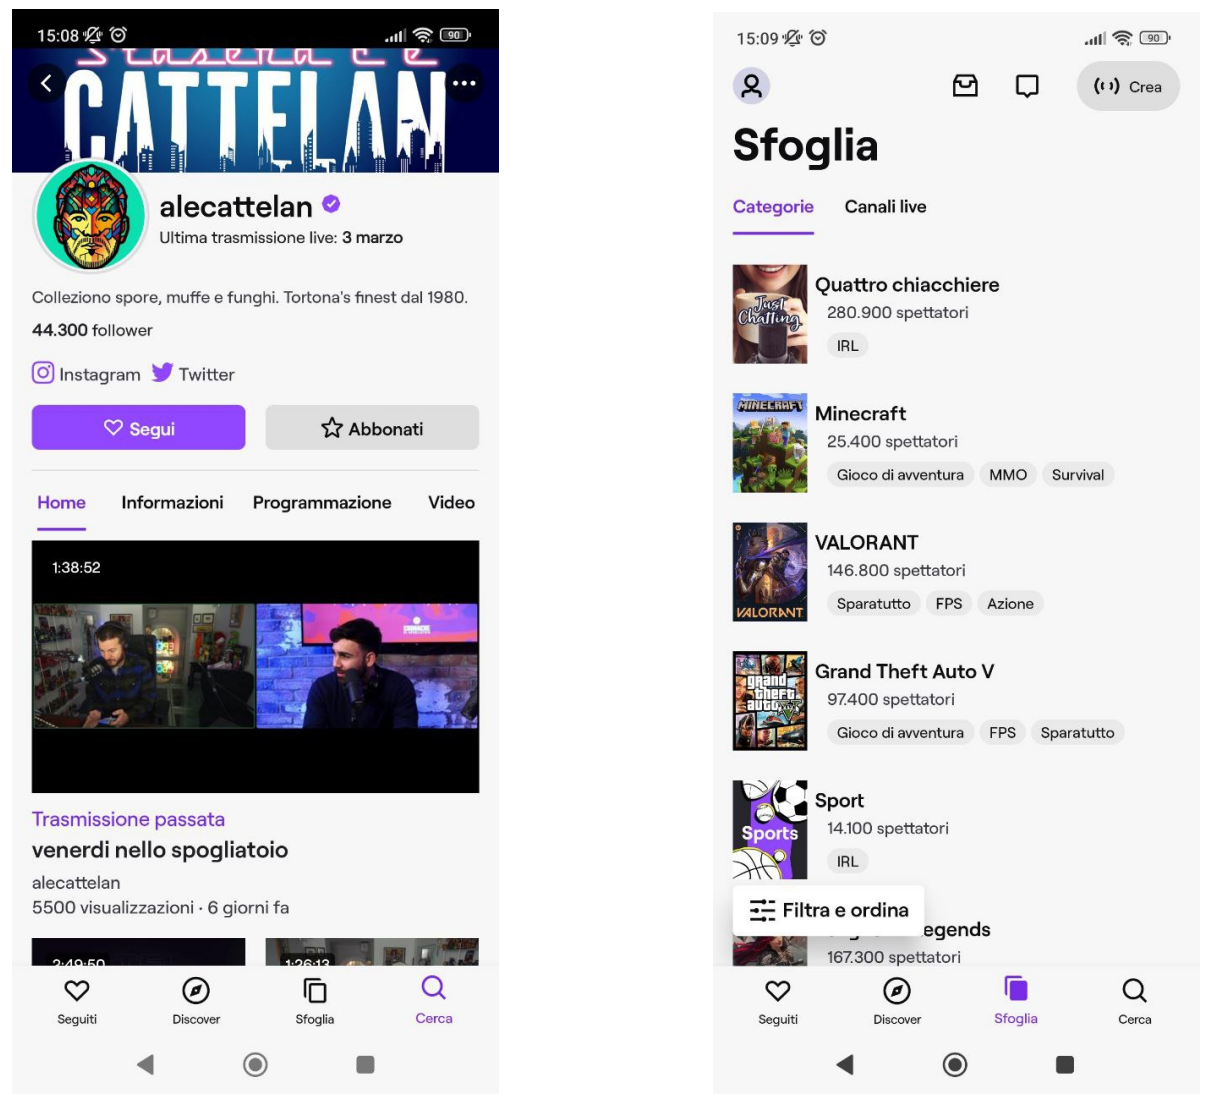
\includegraphics[width=0.5\linewidth]{img/twitch.png}
\end{figure}

Per ogni creatore di contenuti, si memorizzano il numero di live effettuate, il numero di minuti
trasmessi, il numero medio di spettatori simultanei. Inoltre, sulla pagina del canale viene
visualizzato il numero di follower.
Quando uno streamer rispetta determinati parametri di performance (un minimo di 500 minuti
trasmessi, una media di tre o più spettatori simultanei, almeno 50 follower), può diventare affiliate.
Le stream hanno degli orari. Ogni streamer ha un calendario in cui può dire quando farà stream e
indicare il titolo delle prossime live.
I viewer possono diventare follower del canale degli streamer che preferiscono, e le loro
preferenze sono raccolte in un elenco di follower a cui possono accedere dal loro profilo. I viewer
possono inoltre supportare gli streamer tramite la subscription (a pagamento) al loro canale,
ottenendo dei privilegi (emoticon personalizzate, ecc.). Inoltre, gli utenti hanno un portafoglio di bit
(moneta virtuale che possono acquistare tramite la piattaforma), che possono usare per fare
donazioni agli streamer.
Oltre a chattare pubblicamente, gli utenti possono scambiarsi messaggi privati.

La base di dati deve supportare le seguenti operazioni:
\begin{itemize}
    \item Una volta al giorno si controllano le condizioni per la qualifica di affiliate.
    \item Una volta a settimana viene calcolata la classifica degli streamer più seguiti.
\end{itemize}
Si può assumere che i contenuti multimediali vengano gestiti da una piattaforma di video hosting e
che quindi sia sufficiente memorizzare un URL.
\restoregeometry



\newgeometry{margin=0.5cm}
\begin{landscape}
\setlength{\parskip}{2em}
\subsection{Glossario dei termini}
\begin{center}
\begin{tabular}{ |p{5cm}|p{7cm}|p{4cm}|p{5cm}|  }
 \hline
 \multicolumn{1}{|c|}{\textbf{Termine}} 
 & \multicolumn{1}{|c|}{\textbf{Descrizione}} 
 & \multicolumn{1}{|c|}{\textbf{Sinonimi}}
 & \multicolumn{1}{|c|}{\textbf{Collegamenti}}\\
 \hline
 Utente & Partecipante della piattaforma & Pubblico & Calendario, Portafoglio bit, Chat pubblica, Chat privata, Canale, Subscription, Donazione\\
 \hline
 Content creator & Creatore di contenuti & Streamer, Creatore di contenuti & Contenuti\\
 \hline
 Affiliato & Partner Twitch & N.D. & Donazione, Subscription\\
 \hline
 Portafoglio bit & Borsellino virtuale di bit & Wallet & Utente\\
 \hline
 VOD & Video on Demand & N.D. & N.D.\\
 \hline
 Clip & Momenti salienti di un VOD & Video di breve durata & N.D.\\
 \hline
 Video & Contenuto video & Live passata & N.D.\\
 \hline
 Contenuti & Materiale contenutistico & N.D. & Content Creator\\
 \hline
 Live streaming & Trasmissione in diretta & Live, Stream & Utente anonimo, Chat pubblica, Content creator\\
 \hline
 Calendario & Programma settimanale & N.D. & Live streaming, Utente\\
 \hline
 Utente anonimo & Anonimo & Viewer & Live streaming\\
 \hline 
 Chat pubblica & Chatroom globale & Chat & Utente, Live streaming\\
 \hline
 Chat privata & Conversazione privata & Chat & Utente\\
 \hline
 Canale & Profilo utente & N.D. & Utente\\
 \hline 
 Subscription & Iscrizione & N.D. & Utente,  Affiliato\\
 \hline
 Donazione & Contributo monetario & N.D. & Utente, Affiliato\\
 \hline
\end{tabular}
\end{center}
\end{landscape}
\restoregeometry

\subsection{Requisiti rivisti e strutturati in frasi omogenee}
\begin{itemize}
    \item La piattaforma per la quale si vuole realizzare una base di dati è destinata ad ospitare contenuti multimediali, in particolare live streaming, video e clip.
    Il live streaming permette di interagire con il pubblico in tempo reale grazie a feed video, chat e altro.
    \item Ogni utente può essere spettatore o streamer, o entrambi. Per registrarsi, gli utenti devono indicare nome utente, password, data di nascita, numero di telefono o indirizzo mail. Gli utenti registrati possono chattare, seguire lo streamer, creare live streaming.
    \item Gli spettatori possono essere registrati al servizio oppure possono guardare le live streaming in modo anonimo. Gli spettatori registrati possono diventare follower del canale degli streamer che preferiscono e le loro preferenze sono raccolte in un elenco di followee a cui possono accedere dal loro profilo. Gli spettatori possono inoltre supportare gli streamer tramite la subscription (a pagamento) al loro canale, ottenendo dei privilegi (emoticon personalizzate, ecc.). Inoltre, gli utenti hanno un portafoglio di bit (moneta virtuale che possono acquistare tramite la piattaforma), che possono usare per fare donazioni agli streamer.
    Oltre a chattare pubblicamente, gli utenti registrati possono scambiarsi messaggi privati.
    \item Per ogni streamer si memorizzano il numero di live streaming effettuate, il numero di minuti trasmessi, il numero di medio di spettatori simultanei. 
    Quando uno streamer rispetta determinati parametri di performance (un minimo di 500 minuti trasmessi, una media di tre o più spettatori simultanei, almeno 50 follower), può diventare \textit{affiliate}.
    Ogni streamer ha un calendario in cui può dire quando farà stream e indicare il titolo delle prossime live streaming. 
    \item Gli streamer hanno ciascuno un canale, che può essere caratterizzato tramite una descrizione. In ogni canale possono esserci live streaming, video (live streaming passate) e clip (video di durata breve). Ognuno ha un titolo, una durata, appartiene a una categoria e può essere associato a diversi tag. Per ogni live streaming viene memorizzato il numero medio di spettatori mentre per i video e le clip il numero di visualizzazioni. Le live streaming possono anche non diventare video del canale. Si può assumere che i contenuti multimediali vengano gestiti da una piattaforma di video hosting e che quindi sia sufficiente memorizzare un URL.
\end{itemize}

\newpage
\newgeometry{margin=0.5cm}
\begin{landscape}
\subsection{Schema E-R principale + business rules}
\vspace{-\parskip} % Elimina lo spazio aggiunto dall'intestazione della subsection
\subsubsection{Schema E-R}
\vspace{-\parskip} % Elimina lo spazio aggiunto dall'intestazione della subsection
\begin{figure}[h]
    \centering
    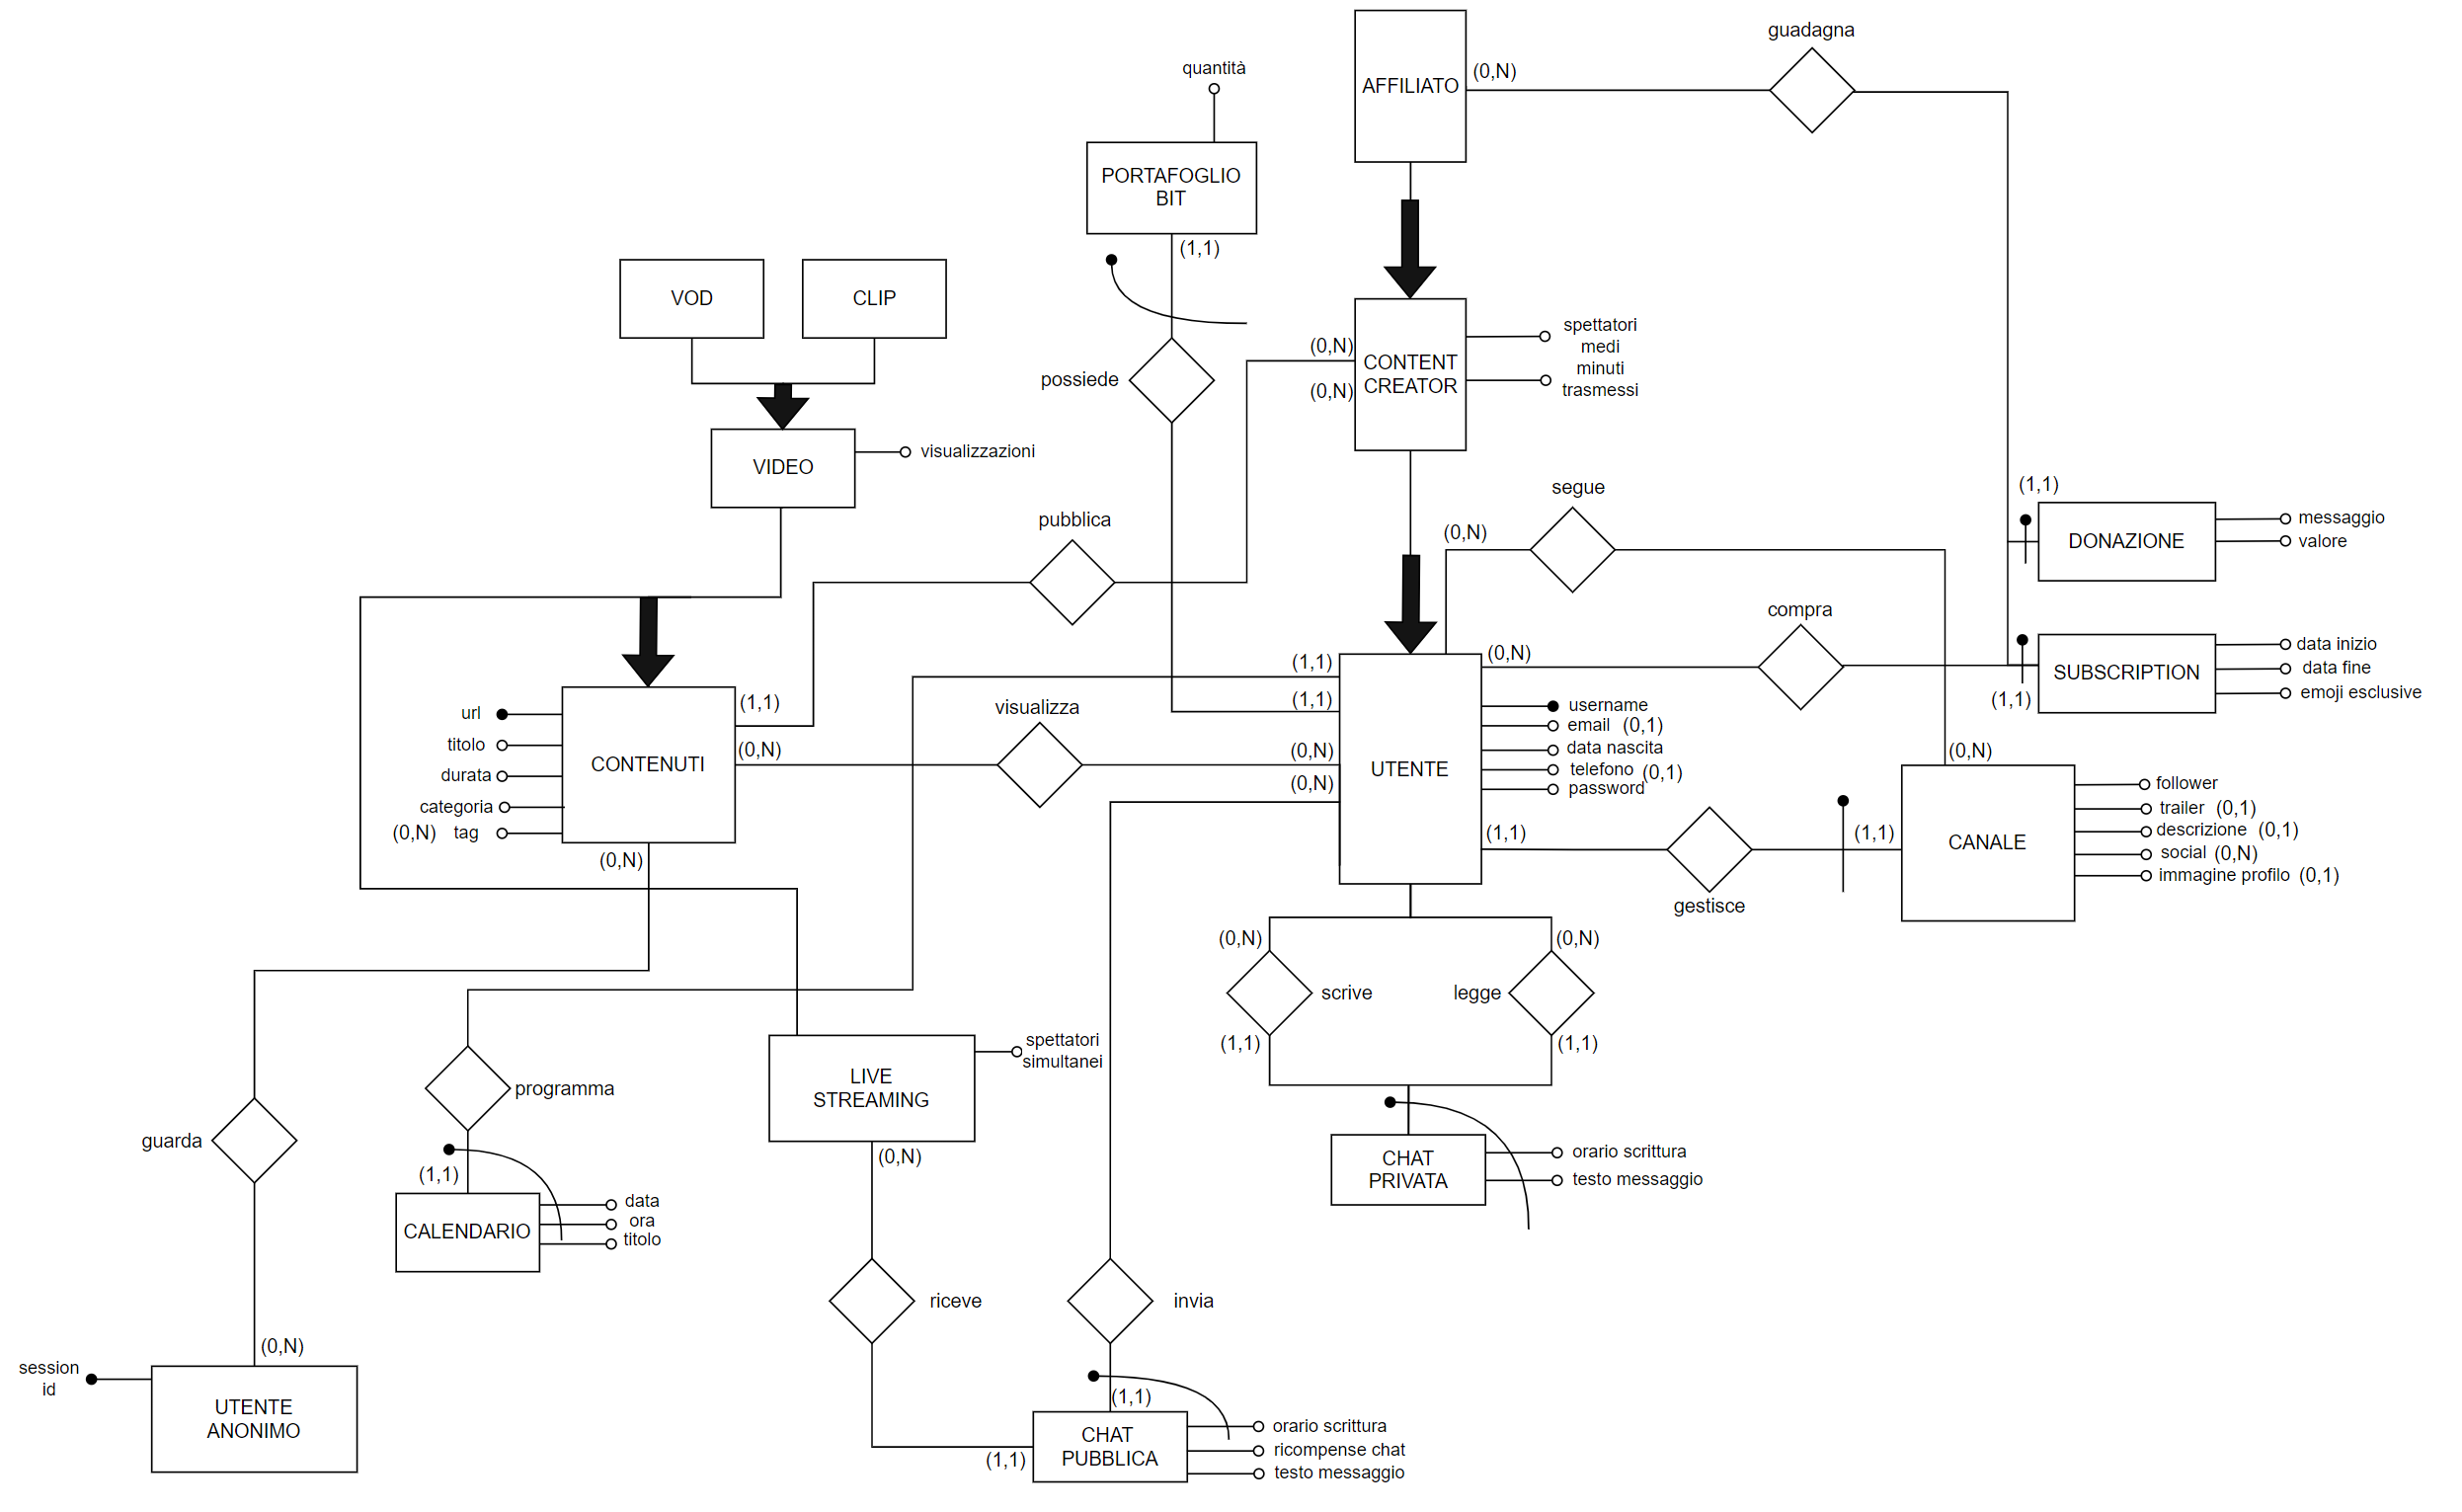
\includegraphics[scale=0.5]{img/ER1.png}
\end{figure}
\end{landscape}
\restoregeometry


\newpage
\setlength{\parskip}{0.5em}
\newgeometry{margin=0.5cm}
\begin{landscape}
\subsubsection{Business Rules}
\subsubsection*{Dizionario dei dati per le entità}
\begin{center}
\begin{tabular}{ |p{5cm}|p{4cm}|p{7cm}|p{5cm}|  }
 \hline
 \multicolumn{1}{|c|}{\textbf{Entità}} 
 & \multicolumn{1}{|c|}{\textbf{Descrizione}} 
 & \multicolumn{1}{|c|}{\textbf{Attributi}}
 & \multicolumn{1}{|c|}{\textbf{Identificatore}}\\
 \hline
 Utente & Partecipante della piattaforma & Username, Email, Data di nascita, Telefono, Password & Username\\
 \hline
 Content creator & Creatore di contenuti & Username, Email, Data di nascita, Telefono, Password, Spettatori medi, Minuti trasmessi & Username \\
 \hline
 Affiliato & Partner Twitch & Username, Email, Data di nascita, Telefono, Password, Spettatori medi, Minuti trasmessi & Username\\
 \hline
 Portafoglio bit & Borsellino virtuale di bit & Quantità & Username\\
 \hline
 Contenuti & Materiale contenutistico & URL, Titolo, Durata, Categoria, Tag & URL \\
 \hline
  Video & Contenuto video & URL, Visualizzazioni, Titolo, Durata, Categoria, Tag & URL \\
 \hline
 VOD & Video on Demand & URL, Visualizzazioni, Titolo, Durata, Categoria, Tag & URL \\
 \hline
 Clip & Momenti salienti di una diretta & URL, Visualizzazioni, Titolo, Durata, Categoria, Tag & URL\\
 \hline
 Live streaming & Trasmissione in diretta & URL, Spettatori simultanei, Titolo, Durata, Categoria, Tag & URL \\
 \hline
 Calendario & Programma settimanale & Data, Ora, Titolo & Data, Ora\\
 \hline
 Utente anonimo & Anonimo & Session id & Session id\\
 \hline 
 Chat pubblica & Chatroom globale & Orario scrittura, Ricompense chat, Testo messaggio & Username, Orario scrittura\\
 \hline
 Chat privata & Conversazione privata & Orario scrittura, Testo messaggio & Username, Orario scrittura, Testo messaggio\\
 \hline
 Canale & Profilo utente & Follower, Trailer, Descrizione, Social, Immagine profilo & Username\\
 \hline 
 Subscription & Iscrizione & Data inizio, Data fine, Emoji esclusive & Username\\
 \hline
 Donazione & Contributo monetario & Messaggio, Valore & Username\\
 \hline
\end{tabular}
\end{center}
\end{landscape}
\restoregeometry








\newpage
\setlength{\parskip}{0.5em}
\newgeometry{margin=0.5cm}
\begin{landscape}
\subsubsection*{Dizionario dei dati per le relazioni}
\begin{center}
\begin{tabular}{ |p{5cm}|p{4cm}|p{7cm}|p{2cm}|  }
 \hline
 \multicolumn{1}{|c|}{\textbf{Relazione}} 
 & \multicolumn{1}{|c|}{\textbf{Descrizione}} 
 & \multicolumn{1}{|c|}{\textbf{Componenti}}
 & \multicolumn{1}{|c|}{\textbf{Attributi}}\\
 \hline
 Possiede & Possesso di un portafoglio di bit & Utente (1,1), Portafoglio bit (1,1) & N.D.\\
 \hline
 Pubblica & Pubblicazione di contenuti & Contenuti (1,1), Content creator (0,N) & N.D. \\
 \hline
 Programma & Invio di un evento nel calendario & Calendario (1,1), Utente (1,1) & N.D.\\
 \hline
 Guarda & Visualizzazione di una diretta da utente anonimo & Utente anonimo (0,N), Contenuti (0,N) & N.D.\\
 \hline
 Visualizza & Visualizzazione di una diretta da utente registrato & Contenuti (O,N), Utente (0,N) & N.D. \\
 \hline
 Riceve & Ricezione di un messaggio pubblico & Live streaming (0,N), Chat pubblica (1,1) & N.D.\\
 \hline
 Invia & Invio di un messaggio pubblico & Utente (0,N), Chat pubblica (1,1) & N.D.\\
 \hline
 Scrive & Scrittura di un messaggio privato & Utente (0,N), Chat privata (1,1) & N.D.\\
 \hline
 Legge & Lettura di un messaggio privato & Chat privata (1,1), Utente (0,N) & N.D.\\
 \hline
 Gestisce & Gestione e possesso di un canale & Utente (1,1), Canale (1,1) & N.D.\\
 \hline
 Compra & Acquisto di una subscription o donazione & Donazione (1,1), Subscription (1,1), Utente (0,N) & N.D.\\
 \hline
 Guadagna & Guadagno di una donazione o di una Subscription & Donazione (1,1), Subscription (1,1), Affiliato (0,N) & N.D.\\
 \hline
 Segue & Follow di un utente verso un canale & Utente (0,N), Canale (0,N) & N.D.\\
 \hline
\end{tabular}
\end{center}
\end{landscape}
\restoregeometry















\subsubsection{Vincoli di Integrità}
\setlength{\parskip}{0.5em}

\begin{itemize}
\item \textbf{Utente:}
  \begin{itemize}
    \item Deve avere un nome utente univoco.
    \item Può seguire altri utenti per ricevere notifiche.
  \end{itemize}

\item \textbf{Content Creator:}
  \begin{itemize}
    \item Può guadagnare denaro tramite pubblicità e abbonamenti.
    \item Deve seguire le linee guida di Twitch.
  \end{itemize}

\item \textbf{Affiliato:}
  \begin{itemize}
    \item Deve rispettare gli accordi di partnership con Twitch.
    \item Può guadagnare una percentuale sui ricavi pubblicitari.
    \item Deve pubblicare contenuti originali.
  \end{itemize}

\item \textbf{Contenuti:}
  \begin{itemize}
    \item I contenuti non devono violare i diritti d'autore.
    \item Devono rispettare le linee guida di Twitch.
  \end{itemize}

\item \textbf{Chat Pubblica:}
  \begin{itemize}
    \item La chat pubblica non deve contenere linguaggio offensivo o contenuti inappropriati.
  \end{itemize}

\item \textbf{Chat Privata:}
  \begin{itemize}
    \item Le chat private non devono essere utilizzate per scopi illegali o dannosi.
  \end{itemize}

\item \textbf{Subscription:}
  \begin{itemize}
    \item Le iscrizioni devono essere ottenute onestamente.
  \end{itemize}

\item \textbf{Donazione:}
  \begin{itemize}
    \item Non si può effettuare una donazione se il portafoglio non contiene bits.
  \end{itemize}
\end{itemize}

